
\subsection*{Data Collection} \label{apndx:data_collection}

\begin{frame}{Setup}
  \begin{itemize}
      \item To simulate the real-world application (nano-satellites), aerial images were necessary.
      \item Images was collected using a light airplane with a thermal camera mounted on it using an in-house designed jig.
      \item A microcontroller was used to trigger the camera acquisitions and save the images in memory.
  \end{itemize}
  \begin{figure}
      \begin{subfigure}[b]{0.49\textwidth}
          \centering
          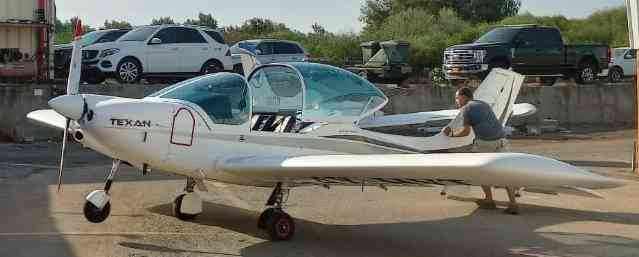
\includegraphics[width=0.8\textwidth]{../figs/data/light_airplane.jpeg}
          \subcaption{Airplane}
          \label{fig:design}
      \end{subfigure}
      \hfill
      \begin{subfigure}[b]{0.49\textwidth}
          \centering
          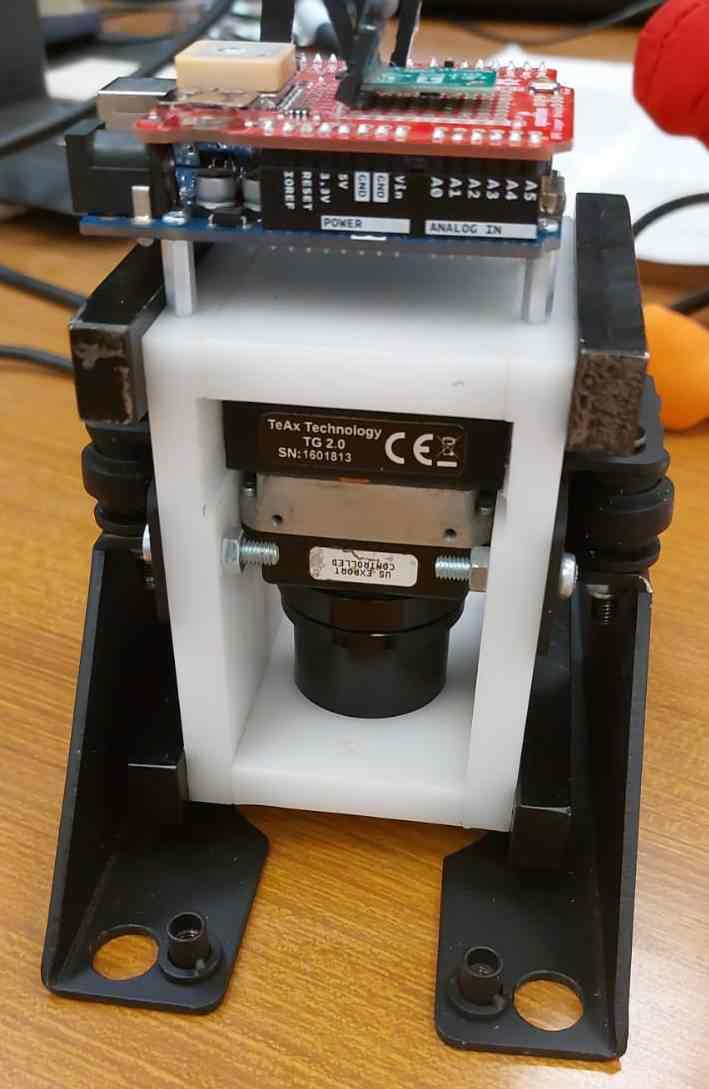
\includegraphics[width=1cm, height=1.5cm]{../figs/data/camera_jig_actual.jpeg}
          \subcaption{Camera Jig}
          \label{fig:manufactured}
      \end{subfigure}
      \label{fig:camera_jig}
  \end{figure}
\end{frame}

\begin{frame}{Data Collection}
\begin{itemize}
      \item The airplane followed a raster trajectory to cover the area of interest.
      \item Several flights were performed, either with an IR filter (monochromatic) or without (monochromatic).
  \end{itemize}
  \begin{figure}
      \centering
      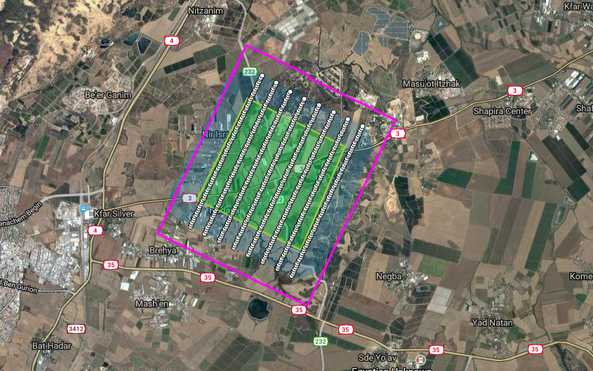
\includegraphics[width=3cm, height=3cm]{../figs/data/aerial_strip.jpeg}
  \end{figure}
\end{frame}


\subsection*{GANs} \label{apndx:gan}
\begin{frame}{Architecture}
  \begin{figure}
    \centering
    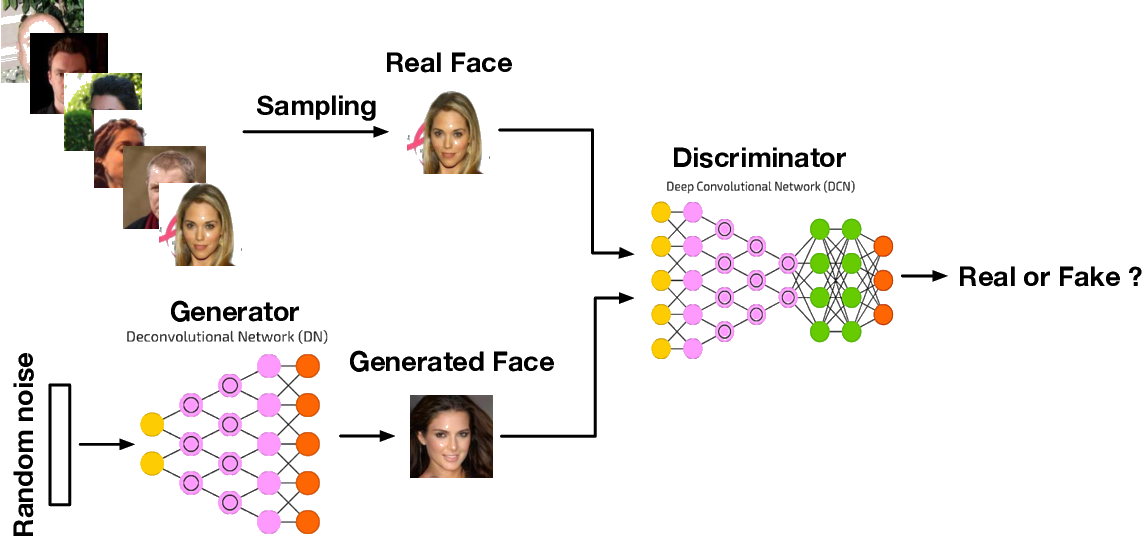
\includegraphics[width=\linewidth]{../figs/related_work/gan_arch.png}
  \end{figure}  
\end{frame}

\begin{frame}{Example}
\begin{itemize}
  \item Able to hallucinate visually appealing fake images. 
  \Eg: this person doesn't exist:
\end{itemize}
\begin{figure}
  \centering
  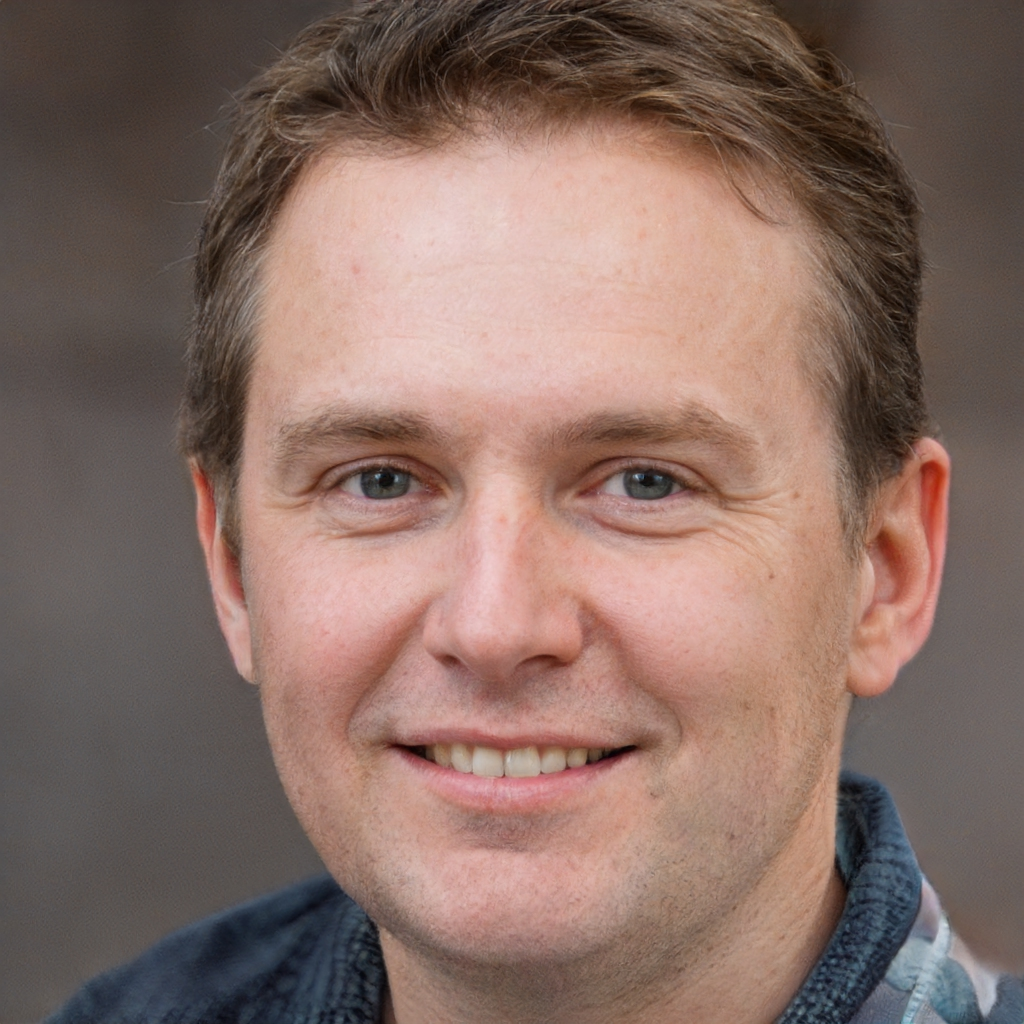
\includegraphics[width=0.5\linewidth]{../figs/related_work/this_person_doesnt_exist.jpg}
\end{figure}  
\end{frame}

\subsection*{Deep UI2I GANs} 
\begin{frame}{CycleGAN} \label{apndx:cycle_gan}
    \begin{itemize}
      \item CycleGAN implements two sets of generators: $A \rightarrow B$ and $B \rightarrow A$.
      \item Spatial consistency is enforcing cycle consistency:
      \begin{equation}
        \mathcal{L}\left( x_A, G_{B \rightarrow A} \left( G_{A \rightarrow B}(x_A) \right) \right) = 
        ||x_A - G_{B \rightarrow A} \left( G_{A \rightarrow B}(x_A) \right)||_1
      \end{equation}
    \end{itemize}
    \begin{figure}
      \centering
      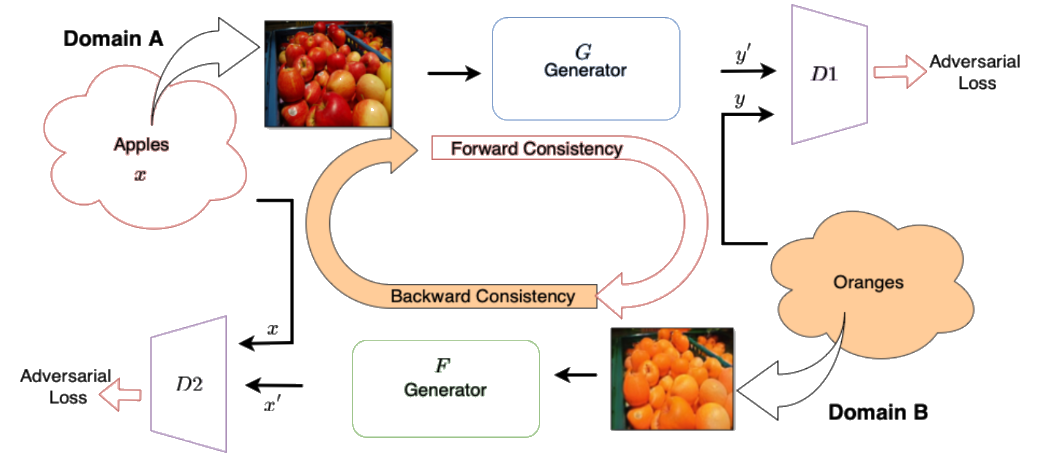
\includegraphics[width=0.8\linewidth]{../figs/related_work/CycleGAN_arch.png}
    \end{figure}  
  \end{frame}
  
  \begin{frame}{CUT} \label{apndx:cat}
    \begin{itemize}
      \item Contrastive Unpaired Translation (CUT) uses a single set of generator and descriminator.
      \item Spatial consistency is enforced by minimizes a patches contrastive loss over between the input and output.
      \begin{figure}
        \centering
        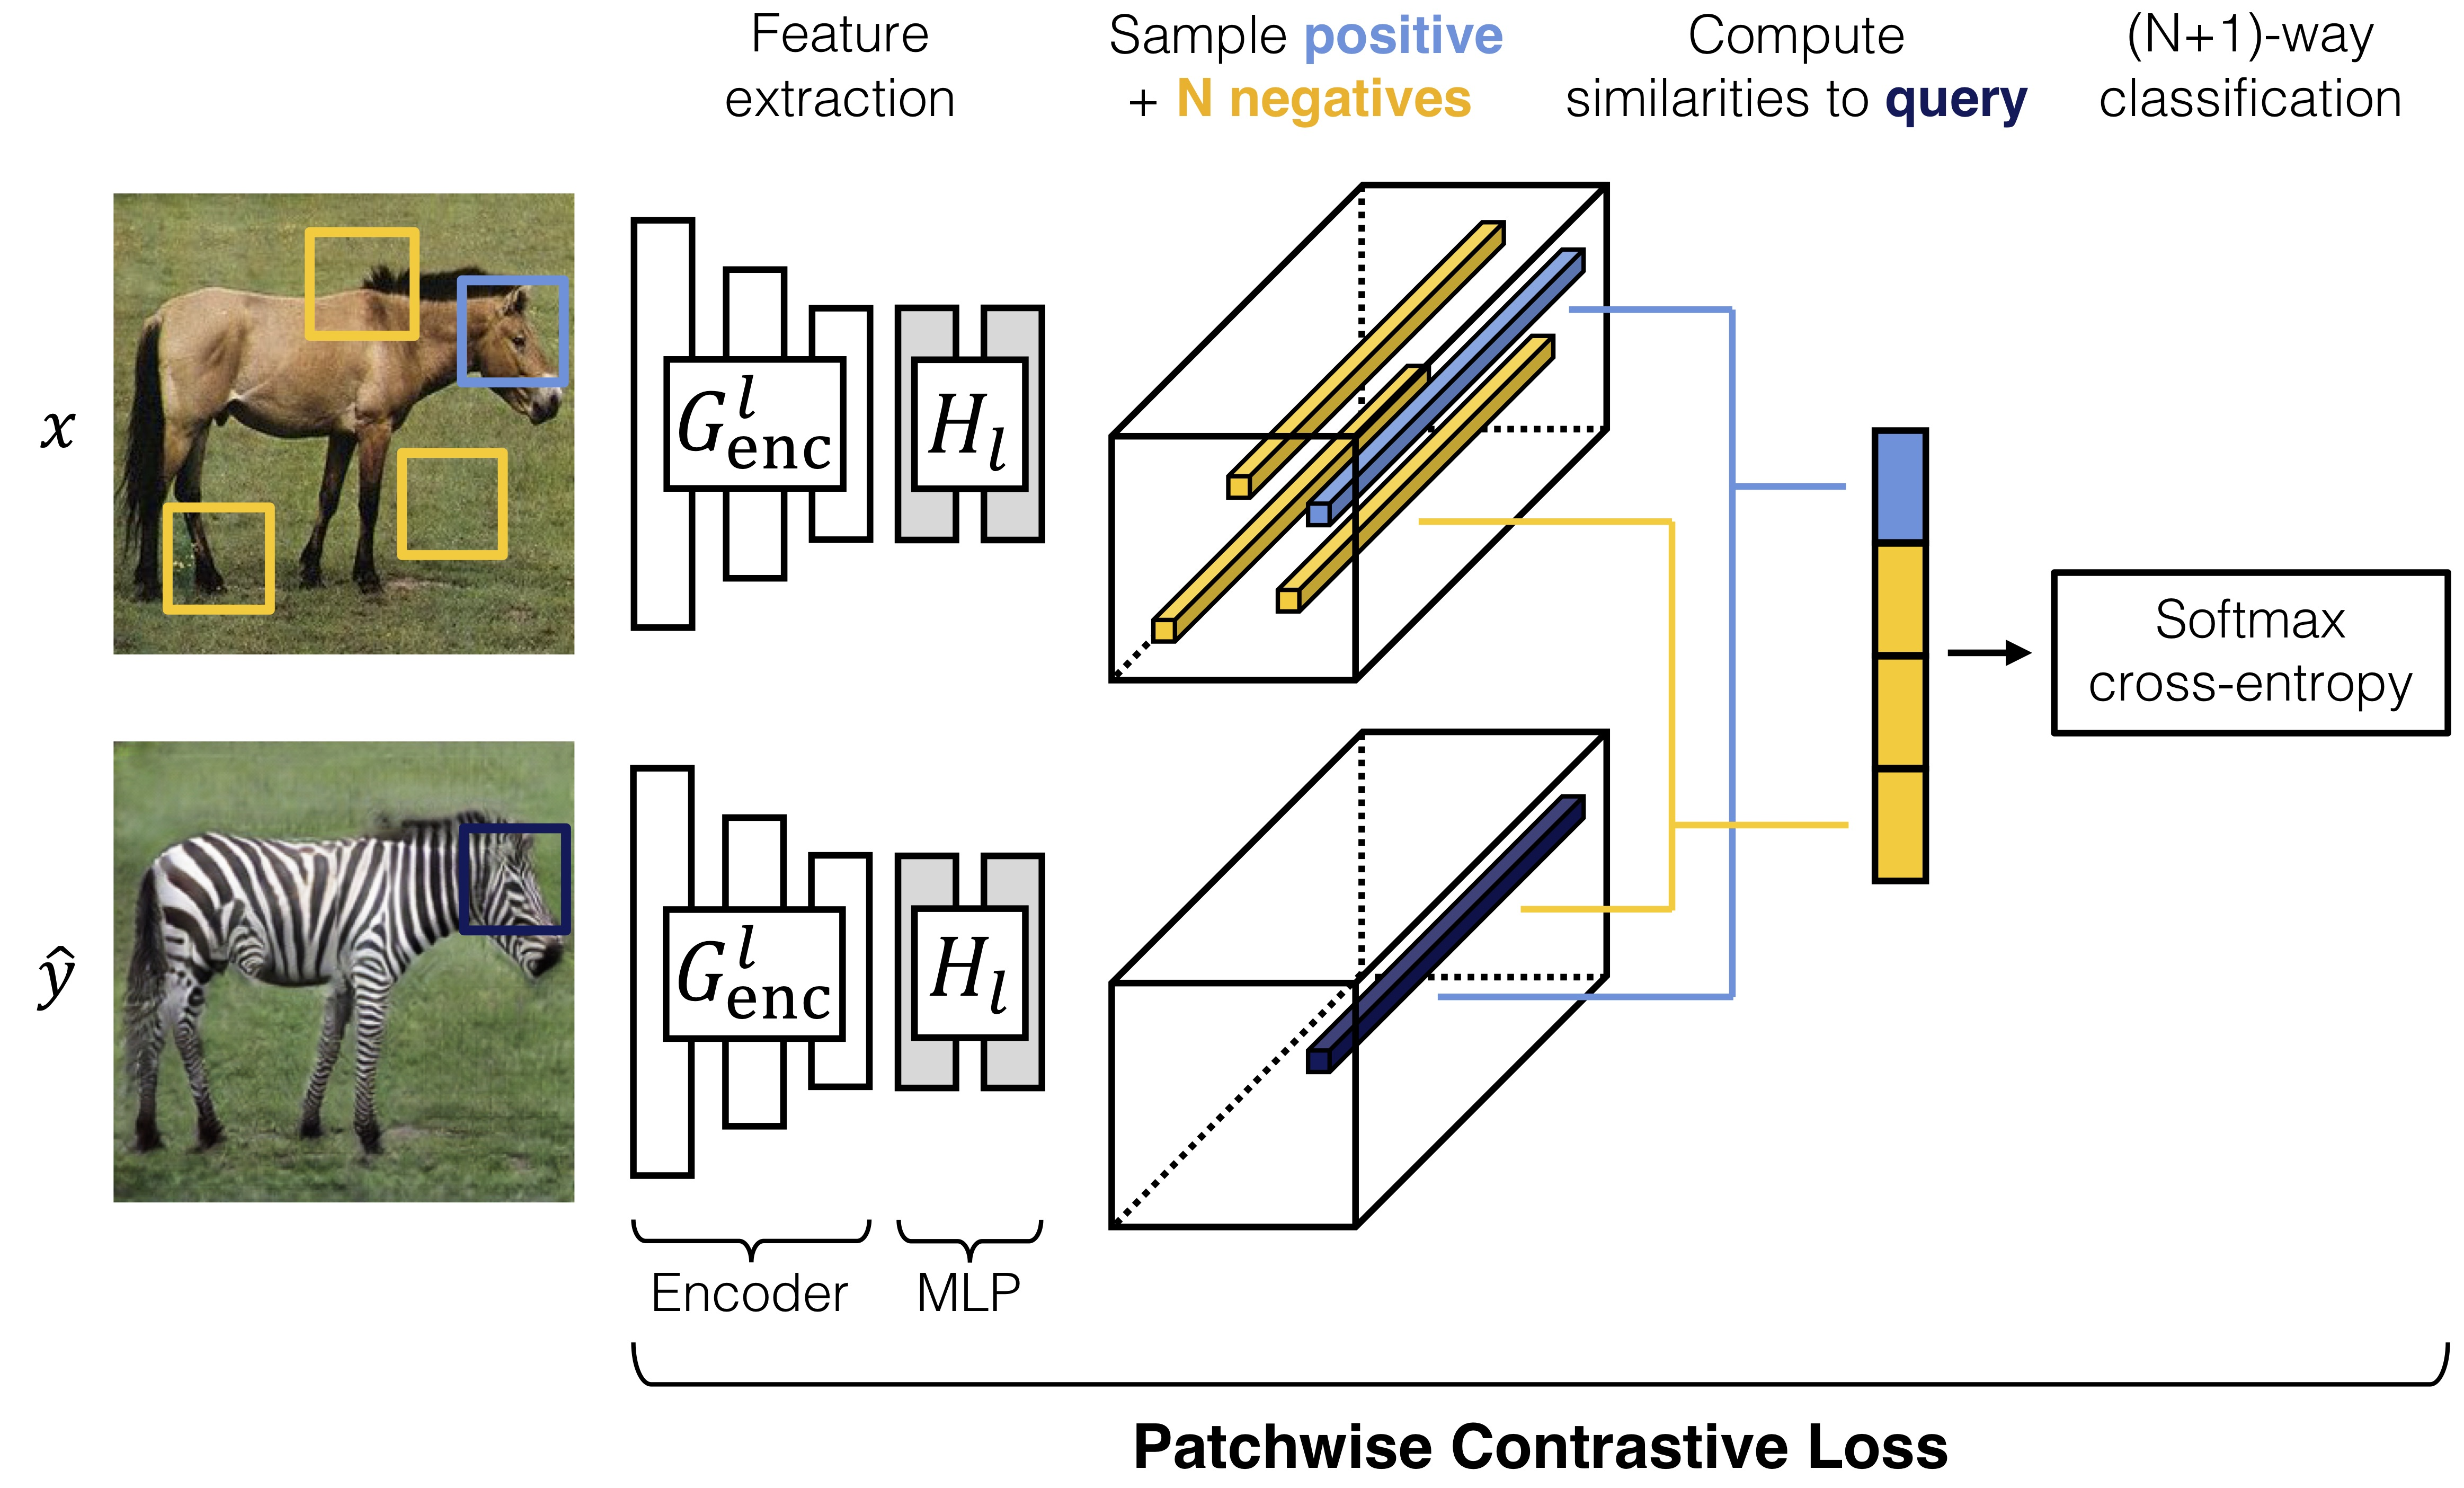
\includegraphics[width=0.8\linewidth]{../figs/related_work/CUT_contrastive_sceheme.png}
        \end{figure}  
    \end{itemize}
  \end{frame}
  